\section{\added{Preliminary Mathematical Methods}}
\label{sec:methods}  % \label{} allows reference to this 

In this Section we review the \added{necessary mathematical tools that we need to formulate our GBD algorithm. This includes the} propagation equations for a single Gaussian beam, \added{how to use} differential ray tracing \added{to compute the parameters necessary} for Gaussian beam propagation, and methods of decomposing the entrance pupil field in the optical system to improve the simulation's sensitivity to high-spatial frequencies. 

\subsection{\added{Propagation of a single Gaussian beam}}
\added{The equation for }a single Gaussian Beam is \added{parameterized} entirely by the complex beam parameter $Q(z)$, \cite{goodman17}
\begin{equation}
	U(r,z) = \frac{U_o}{Q(z)}exp\Bigl[ik\frac{r^2}{2Q(z)}\Bigr],
\end{equation}
where \added{$U(r,z)$ is the scalar Gaussian field,} $U_o$ is the amplitude, $k$ is the wavenumber, and $r$ is the radial coordinate in the plane perpendicular to propagation. The \added{inverse of the} complex parameter $Q(z)$ describes the beam's $1/e$ field radius (the ``waist" $w(z)$) and wavefront radius of curvature $R(z)$,
\begin{equation}
	Q(z)^{-1} = \frac{1}{R(z)}+i\frac{\lambda}{\pi w(z)^2}.
\end{equation}	
$Q(z)^{-1}$ is a convenient expression of the Gaussian beam because it fully encapsulates the information required to describe the transverse electric field of the beam as it propagates. The real part of $Q(z)^{-1}$ is related to the radius of curvature of the wavefront,
\begin{equation}
    R(z) = z\Bigl(1+(\frac{Z_o}{z})^2\Bigr),
    \label{eq:complex_curvature}
\end{equation}
where $Z_o$ is the Rayleigh range and $z$ is the longitudinal propagation distance.
The imaginary part of $Q(z)^{-1}$ is related to the beam waist radius,
\begin{equation}
	w(z) = w_o\sqrt{1+\Bigl(\frac{z}{Z_o}\Bigr)^2}.
\end{equation}
In the paraxial regime $Q(z)^{-1}$ can be propagated using the ABCD ray transfer matrices of geometrical optics\added{\cite{Siegman_1986}}.
\begin{equation}
    Q(z)^{-1}_{2} = \frac{C + DQ_{1}^{-1}}{A + BQ_{1}^{-1}}
    \label{eq:propq}
\end{equation}
\added{To account for system misalignments}, $Q(z)^{-1}$ is a 2x2 matrix $\textbf{Q}(z)^{-1}$ that encodes the complex curvature in two orthogonal directions and how they couple into each other\added{, allowing for the beamlet to be generally astigmatic.}\cite{Ashcraft2020,cai_decentered_nodate}. 

\begin{equation}
    \textbf{Q}(z)^{-1} = 
    \begin{pmatrix}
    Q(z)_{xx}^{-1} & Q(z)_{xy}^{-1} \\
    Q(z)_{yx}^{-1} & Q(z)_{yy}^{-1} \\
    \end{pmatrix}
\end{equation}

This treatment allows for greater versatility in the beamlet propagation, but requires that the elements of the ray transfer matrices are also 2x2 matrices. The propagation formula shown in Equation \ref{eq:propq} has a similar matrix extension.

\begin{equation}
    \mathbf{Q}(z)_{2}^{-1} = (\mathbf{C} + \mathbf{DQ}^{-1}_{1})(\added{\mathbf{A}} + \mathbf{\added{B}Q}^{-1}_{1})^{-1}
    \label{eq:prop_complex}
\end{equation}

\added{We can then express the propagated Gaussian beam with Equation \ref{eq:gaussian_prop}}
\begin{equation}
    U(\mathbf{r}) = \frac{U_{o}}{\sqrt{det|\mathbf{A} + \mathbf{BQ_{1}^{-1}}|}} exp\Bigl[\frac{-ik}{2} \mathbf{r}^{T} \mathbf{Q_{2}^{-1}} \mathbf{r}\Bigr],
    \label{eq:gaussian_prop}
\end{equation}

\added{Where $\mathbf{r}$ is the radial coordinate in the plane transverse to the propagation direction centered on the Gaussian beam.} The formulation for the propagation of the complex curvature matrix allows for modeling Gaussian beams as they propagate along generally skew ray paths in non-axially symmetric optical systems. This is an important utility for diffraction modeling of wavefront aberrations introduced by system misalignment or thermal deformations, which generally break optical system symmetry. \added{Note that the solution in Equation \ref{eq:gaussian_prop} is only valid for propagation between planes that are orthogonal to the propagation direction of the Gaussian beam \cite{Collins:70}. We next need to determine a method for computing the ray transfer matrix for an arbitrary ray path through an optical system in order to propogate the Gaussian beam.}

\subsection{Computing the Differential Ray Transfer Matrix}
The ABCD ray transfer matrix is a useful and concise method for analyzing properties of ray paths along optical systems. In the regime of geometrical optics, a generally skew ray can be traced through a system using 4x4 ABCD ray transfer matrices\cite{Brouwer64}. These matrices model simple optical elements (e.g. thin lenses) with ease by operating on an input column vector that represents a light ray. The simplest ray transfer matrix that describes a paraxial and orthogonal optical system is a 2x2 operator that maps an input ($i$) spatial and angular coordinate to the appropriate output ($o$),
\begin{equation}
    \begin{pmatrix}
    y_o \\
    m_o \\
    \end{pmatrix}
    =
    \begin{pmatrix}
    A & B \\
    C & D \\
    \end{pmatrix}
    \begin{pmatrix}
    y_i \\
    m_i \\
    \end{pmatrix},
\end{equation}
where $y$ is the spatial coordinate transverse to the propagation direction, and $m$ is the slope in that dimension. The elements of the ABCD matrix and ray vectors are real-valued scalars. To account for skew ray paths, the position and angle in the dimension orthogonal to $y$ and the direction of propagation must be tracked, adding two dimensions to the matrix calculus. A 4x4 ABCD matrix describes a nonorthogonal system with tilts and decenters that map generally skew input rays to generally skew output rays, 

\begin{equation}
    \begin{pmatrix}
    x_o \\
    y_o \\
    l_o \\
    m_o \\
    \end{pmatrix}
    = 
    \begin{pmatrix}
    A_{xx} & A_{xy} & B_{xx} & B_{xy} \\
    A_{yx} & A_{yy} & B_{yx} & B_{yy} \\
    C_{xx} & C_{xy} & D_{xx} & D_{xy} \\
    C_{yx} & C_{yy} & D_{yx} & D_{yy} \\
    \end{pmatrix}
    \begin{pmatrix}
    x_i \\
    y_i \\
    l_i \\
    m_i \\
    \end{pmatrix}.
    \label{eq:totalabcdmatrix}
\end{equation}

For simplicity, it is convenient to represent \added{the} radial position in the plane transverse to propagation ($x$, $y$) and the corresponding direction in the dimension ($l$, $m$) as a position and angle vector respectively ($\mathbf{r}, \boldsymbol{\theta}$). The ABCD matrix can similarly be condensed into 2x2 sub matrices that operate on each spatial dimension, yielding a familiar notation,
\begin{equation}
    \begin{pmatrix}
    \mathbf{r_{o}} \\
    \boldsymbol{\theta_{o}} \\
    \end{pmatrix}
    =
    \begin{pmatrix}
    \mathbf{A} & \mathbf{B} \\
    \mathbf{C} & \mathbf{D} \\
    \end{pmatrix}
    \begin{pmatrix}
    \mathbf{r_{i}} \\
    \boldsymbol{\theta_{i}} \\
    \end{pmatrix}
    \label{eq:matrixabcd}.
\end{equation}

This description is powerful because it communicates the elegance and simplicity of ray transfer matrices. All dimensions transverse to propagation are accounted for, but the calculus to propagate a ray is still the same. The ray transfer matrices for simple and paraxial optical elements (e.g. thin lens) are well known\cite{Brouwer64}, and were used in concert with GBD in a prior investigation with paraxial systems\cite{Ashcraft2020}. However, our aim is to use GBD to model \emph{non}-paraxial optical system diffraction. Therefore, we need a method of computing the ray transfer matrix for \added{an arbitrary } skew ray-path. 
A simple dimensional analysis of the matrix relation in Equation \ref{eq:matrixabcd} is a good place to start understanding how to construct an arbitrary ABCD matrix. Because the position element $\mathbf{r}$ of the ray vector must be in units of distance, and the angular element $\boldsymbol{\theta}$ must be dimensionless, the units of the ABCD matrix elements are constrained. $\mathbf{A}$ and $\mathbf{D}$ must be dimensionless and transform the ray position and angle through the optical system, indicating that they represent magnification. $\mathbf{B}$ and $\mathbf{C}$ must have units of distance and inverse distance, respectively. $\mathbf{B}$ operates on an angle, and is therefore a metric of propagation distance through an optical system given some ray angle. $\mathbf{C}$ operates on a position, and is therefore an indicator of the amount of refraction a ray experiences given a position in the entrance pupil.

Stone and Forbes'\cite{Stone:97} work in differential ray tracing for inhomogeneous media was instructive in terms of deriving a method to construct the ABCD matrix. They illustrate the construction of individual optical elements through ray derivatives in a generally 4x4 matrix through derivatives of surface data. Using this method the position and angular derivatives of an optical surface are taken and arranged in a matrix like in Equation \ref{eq:matrixabcd}. The matrix product of the optical elements is then the final differential ray transfer (or ABCD) matrix. Their method is functional if the analytical expression of the optical elements are known, but could be very computationally intensive if the optical system has many elements. Instead, we approximate the differential matrix by tracing additional rays, and compute the finite difference of the ray coordinates and directions at the input and output of the optical system to approximate the derivative.

Our implementation \added{of the differential ray tracing technique in Poke} utilizes \added{a user-specified ray tracer (e.g. Zemax OpticStudio)} that propagates rays by computing Snell's law at each surface. \added{For GBD, the ray coordinates of interest are on the source plane (where the field decomposition is done, e.g. the entrance pupil) and the transversal plane. The transversal plane is the plane normal to the central ray of a Gaussian beam that intersects the point at which we wish to evaluate the field. Propagation to this plane is critical, because the solution to Gaussian beam propagation (Equation \ref{eq:gaussian_prop}) is only valid between planes orthogonal to the propagation direction defined by the central ray.} \added{An element of the ray transfer matrix can be computed by determining the ratio of the differential ray data on the transversal plane to the differential ray data on the source plane.} An example of computing the element \added{$A_{yy}$} is given by Equation \ref{eq:Ayy}, 

\begin{equation}
    A_{yy} = \added{\frac{\partial y_{T}}{\partial y_{S}} = \frac{y_{+y,T} - y_{cen,T}}{y_{+y,S} - y_{cen,S}}.}
    \label{eq:Ayy}
\end{equation}

\added{Where $y_{+y,T}$, and $y_{cen,T}$ are the ray coordinates of the differential ray and the central ray, respectively, on the transversal plane. $y_{+y,S}$, and $y_{cen,S}$ are the coordinates of the same rays on the source plane.}  In this example the central ray (shown in black on Figure \ref{fig:diffdiagram}) is traced along with a ray with a differential addition in input \added{$y$} coordinate (shown in red on Figure \ref{fig:diffdiagram}). The \added{difference in} \added{$y$} coordinates of the \added{central and $\delta y$ differential ray determine the derivative}. 

\begin{figure}[H]
    \centering
    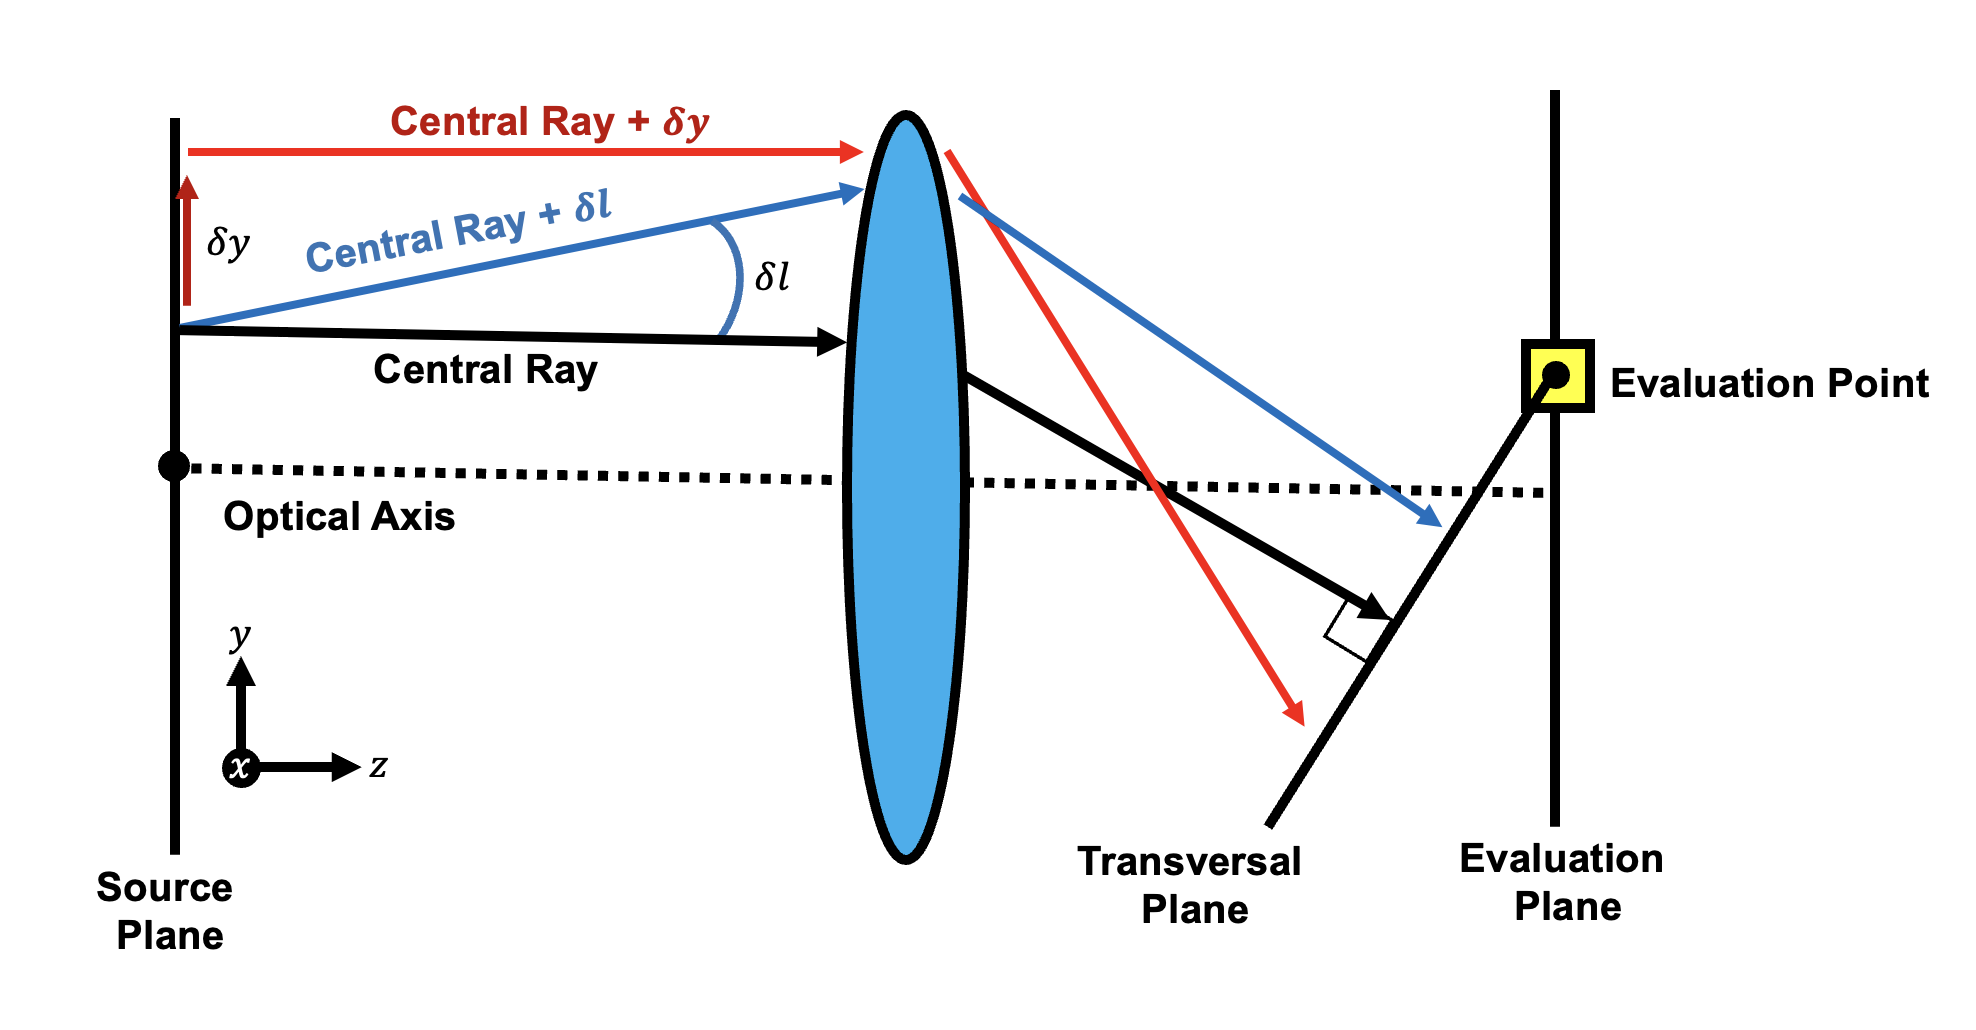
\includegraphics[width=0.8\textwidth]{differential_diagram_2.png}
    \caption{Diagram illustrating differential ray tracing in the 2D case for a simple lens system. The central ray (black) is propagated along with two parabasal rays with a differential addition in the $y$ direction (red) and another with a differential addition in the $l$ direction (blue). To determine the ABCD matrix the ray data is computed on the transversal plane, which is normal to the central ray \added{and intersects the point at which we wish to evaluate the field.}}
    \label{fig:diffdiagram}
\end{figure}

The ray transfer matrix for a non-orthogonal optical system has 16 unknowns \added{(see ABCD matrix in Equation \ref{eq:totalabcdmatrix})}, and each ray yields 4 quantities. To solve for every element of the matrix 4 linearly independent rays must be traced. The simplest ray set is geometrically orthogonal\cite{Greynolds86}, where copies of the central ray $(x,y,l,m)$ are modified by a differential quantity $(\delta)$ in each of the 4 ray coordinates, \added{two in position ($\delta x$, $\delta y$) and two in slope ($\delta l$, $\delta m$)}. The differential ray set is given by Equation \ref{eq:diffrays}
\begin{center}
    
\begin{equation}
    \begin{pmatrix}
    x + \delta x \\
    y \\
    l \\
    m \\
    \end{pmatrix}
    ,
    \begin{pmatrix}
    x \\
    y + \delta y \\
    l \\
    m \\
    \end{pmatrix}
    ,
    \begin{pmatrix}
    x \\
    y \\
    l + \delta l\\
    m \\
    \end{pmatrix}
    ,
    \begin{pmatrix}
    x \\
    y \\
    l \\
    m + \delta m\\
    \end{pmatrix},
    \label{eq:diffrays}
\end{equation}

\end{center}
\added{which are traced in addition to} the \added{central} ray of interest\added{.} The full differential ray transfer matrix is given by Equation \ref{eq:diffmat_rays}. The ray transfer matrix is purely a function of the Cartesian position of the ray ($x, y$) and  slope of the ray in those directions ($l, m$) at the input and output of the optical system. \added{An example of propagating a ray from the source plane to the transversal plane is shown in Equation \ref{eq:diffmat_rays}. Here the subscript $S$ refers to the coordinate on the source plane, and the subscript $T$ refers to the coordinate on the transversal plane. The elements of Equation \ref{eq:diffmat_rays} are computed in a similar fashion to the example in Equation \ref{eq:Ayy}, but with different ray data.}


\begin{center}
\begin{equation}
    \begin{pmatrix}
    x_{T} & y_{T} & l_{T} & m_{T} \\
    \end{pmatrix}
    =
    \begin{pmatrix}
    \frac{\partial x_T}{\partial x_S} & \frac{\partial x_T}{\partial y_S} & \frac{\partial x_T}{\partial l_S} & \frac{\partial x_T}{\partial m_S}  \\
    \frac{\partial y_T}{\partial x_S} & \frac{\partial y_T}{\partial y_S} & \frac{\partial y_T}{\partial l_S} & \frac{\partial y_T}{\partial m_S}  \\
    \frac{\partial l_T}{\partial x_S} & \frac{\partial l_T}{\partial y_S} & \frac{\partial l_T}{\partial l_S} & \frac{\partial l_T}{\partial m_S} \\
    \frac{\partial m_T}{\partial x_S} & \frac{\partial m_T}{\partial y_S} & \frac{\partial m_T}{\partial l_S} & \frac{\partial m_T}{\partial m_S} \\
    \end{pmatrix}
    \begin{pmatrix}
    x_S \\
    y_S \\
    l_S \\
    m_S \\
    \end{pmatrix}
    %$
    \label{eq:diffmat_rays}
\end{equation}
\end{center}
 
\added{With differential ray tracing we are able to propagate a single Gaussian beam through an arbitrary optical system using the ABCD matrix. To perform GBD, we next need to understand how to decompose the field in the entrance pupil of the optical system.}

\subsection{Entrance Pupil Spatial Decomposition}
\added{The final variable to constrain in GBD is how to appropriately decompose the field in the entrance pupil into a finite set of Gaussian beams. This problem is illustrated in 1D earlier in Figure \ref{fig:gbd_essentials}; however, for imaging systems the decomposition is a 2D problem.} The fundamental \added{Gaussian mode} does not represent a complete set\cite{koshel_novel_2001}, and therefore the decomposition of the field is not unique. We must carefully consider how the beamlets are distributed in the entrance pupil for accurate diffraction calculations. 

Various \added{sampling} schemes exist in the literature, with different strengths and weaknesses. The \emph{even Cartesian} \added{sampling} scheme (shown on the left in Figure \ref{fig:sampleschemes}) described in Harvey et al\cite{Harvey15} is the most straightforward, where the beamlets lie evenly spaced along a Cartesian grid. The ray coordinates in the entrance pupil are then computed from an overlap factor (OF) which describes the overlap of the beamlets\added{'} $1/e$ waist radii $w_o$,
\begin{equation}
    OF = \frac{N_{g} 2 \omega_{o}}{W},
\end{equation}
where $N_{g}$ is the number of Gaussian beamlets across an aperture, and $W$ is the width of the aperture. This feature is easy to implement and understand, but for under-sampled cases it introduces artifacts due to the ripple from the distribution and soft edge left by the Gaussian beamlets. 

The \emph{Fibonacci} \added{sampling} scheme (shown in the middle in Figure \ref{fig:sampleschemes}) introduced by Worku and Gross places the beamlets along a Fibonacci spiral, which results in a more accurate decomposition for circular apertures\cite{Worku:18}. The distribution of the beamlets is even along polar angles on the spiral. The polar distribution of the beamlets is given by a position $R$ and angle $\Theta$,
\begin{equation}
    R = \frac{W}{2}\sqrt{N_{g}},
\end{equation}
\begin{equation}
    \Theta = \frac{2\pi}{\phi^{2}}N_{g},
\end{equation}
where $\phi$ is the golden ratio and $N_{g}$ is the total number of beamlets to trace. Even polar sampling (shown on the right in Figure \ref{fig:sampleschemes}) is also a viable method to increase the accuracy of the decomposition for fewer beamlets assuming the optical system has a circular aperture\cite{Worku:18}, but was not explored in this study due to the apparent advantages of the Fibonacci sample scheme, which are shown in \hyperref[sec:results]{Section \ref{sec:results}} \added{.}

\begin{figure}[H]
    \centering
    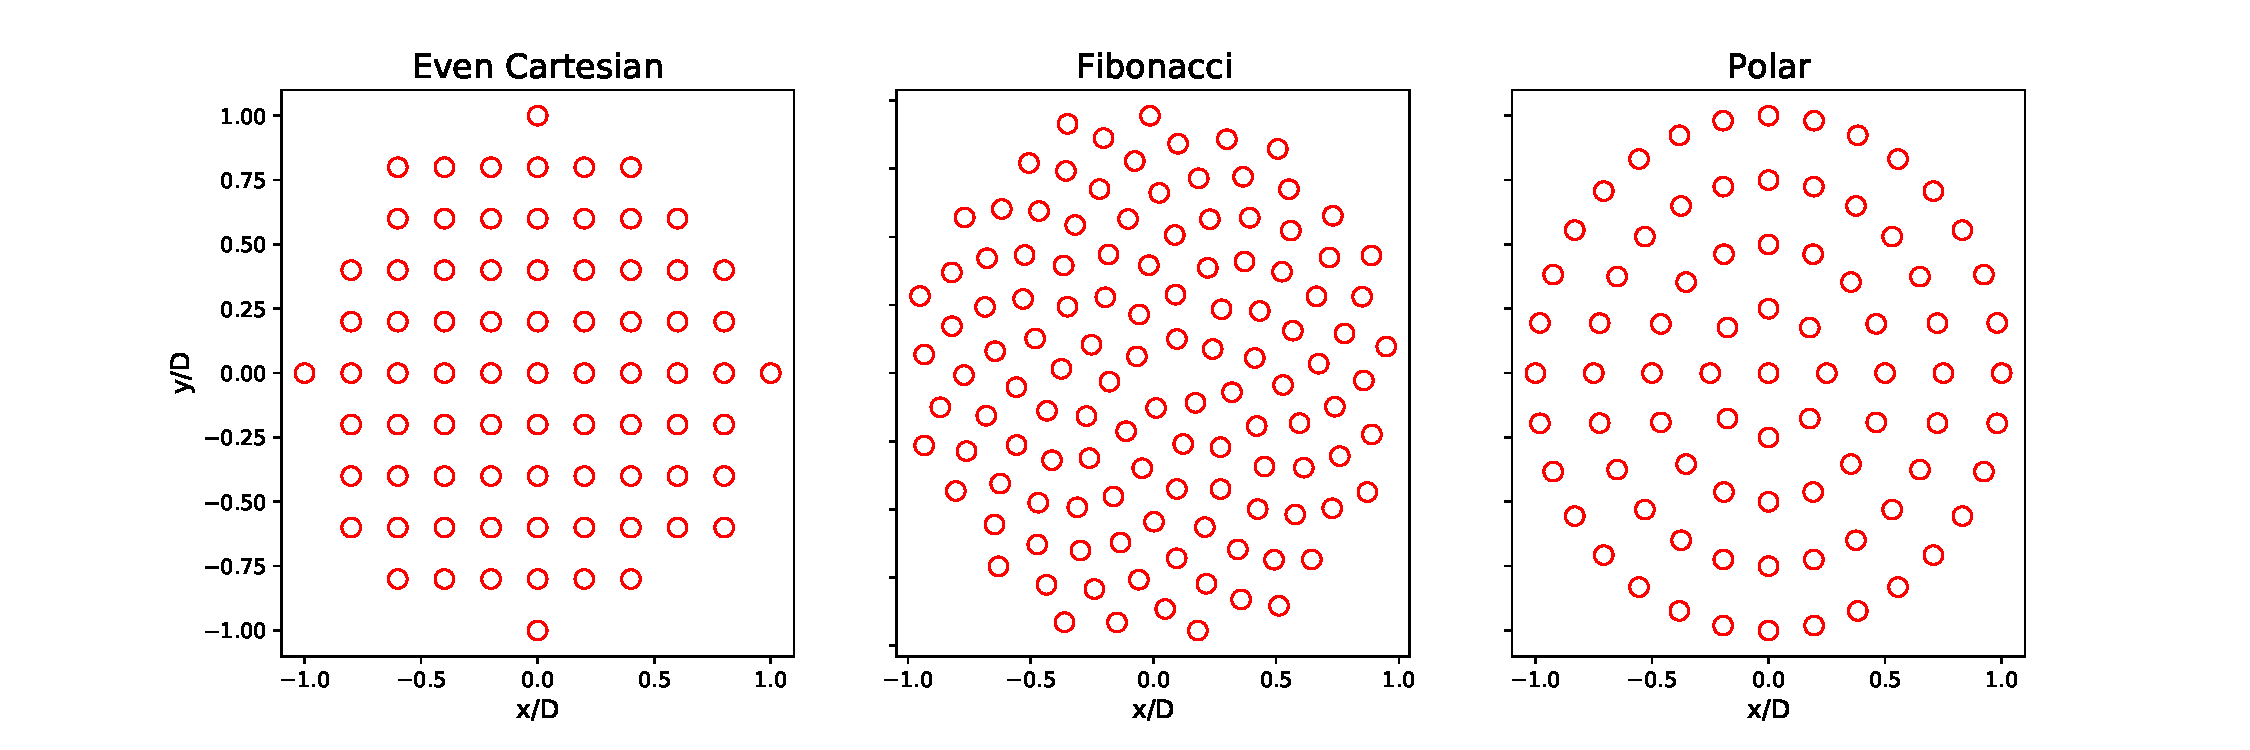
\includegraphics[width=\textwidth]{sampleschemes.pdf}
    \caption{Illustration of the Even (left), Fibonacci (middle), and Polar (right) sample schemes for decomposing the field at the entrance pupil of the optical system with approximately the same number of beamlets in each Figure. Quantifying the ramifications of these \added{sampling} schemes is of paramount importance to accurate diffraction simulation.}
    \label{fig:sampleschemes}
\end{figure}

